% Copyright (C) 2020 - Michael Baudin

% \documentclass{beamer}
\documentclass[aspectratio=169]{beamer}
%\setbeameroption{hide notes}
%\setbeameroption{show notes}
%\setbeameroption{show only notes}

% Copyright (C) 2012 - EDF R&D - Michael Baudin

% To highlight source code
\usepackage{listings}
\definecolor{darkgreen}{rgb}{0,0.5,0}
\definecolor{violet}{rgb}{0.5,0,1}

\usepackage{lmodern}% http://ctan.org/pkg/lm

\usetheme{Montpellier}
\setbeamertemplate{navigation symbols}{} % Remove navigation
\useoutertheme{infolines}

\usepackage[utf8]{inputenc}
\usepackage[T1]{fontenc}

\usepackage{graphicx}
\unitlength=1cm
\graphicspath{{./figures/}}

\usepackage{hyperref}
\hypersetup{colorlinks=true, linkcolor=blue, linktocpage, urlcolor=blue}

\def\bx{{\bf x}}
\def\RR{\mathbb{R}}

\newcommand{\pyvar}[1]{\texttt{#1}}

\def \ot {OpenTURNS}

\definecolor{codegreen}{rgb}{0,0.6,0}
\definecolor{codegray}{rgb}{0.5,0.5,0.5}
\definecolor{codepurple}{rgb}{0.58,0,0.82}
\definecolor{backcolour}{rgb}{0.95,0.95,0.92}
\lstdefinestyle{mystyle}{
  backgroundcolor=\color{backcolour},   commentstyle=\color{codegreen},
  keywordstyle=\color{magenta},
  numberstyle=\tiny\color{codegray},
  stringstyle=\color{codepurple},
  basicstyle=\ttfamily\tiny,
  breakatwhitespace=false,         
  breaklines=true,                 
  captionpos=b,                    
  keepspaces=true,                 
  numbers=left,                    
  numbersep=5pt,                  
  showspaces=false,                
  showstringspaces=false,
  showtabs=false,                  
  tabsize=1,
  numbers=none
}

\lstset{style=mystyle, language=python}


\title[PERSALYS]{PERSALYS, the graphical interface of OpenTURNS}

\author[PERSALYS Team]{
M. Baudin \inst{1} \and
A. Dumas \inst{2} \and
A. Dutfoy \inst{1} \and \\
\underline{G. Garcia} \inst{2} \and
O. Mircescu \inst{1} \and
J. Mure \inst{1} \and
J. Pelamatti \inst{1} \and \\
J. Schueller \inst{2} \and
T. Yalamas \inst{2}
}

\institute[EDF-Phimeca]{
\inst{1} EDF R\&D. 6, quai Watier, 78401, Chatou Cedex - France, michael.baudin@edf.fr \and %
\inst{2} Phimeca Engineering. 18/20 boulevard de Reuilly, 75012 Paris - France, yalamas@phimeca.com
}

\date[]{June 23th 2023, OpenTURNS User's day}

%%%%%%%%%%%%%%%%%%%%%%%%%%%%%%%%%%%%%%%%%%%%%%%%%%%%%%%%%%%%%%%%%%%%%%%%%%%%%

  \begin{document}

%%%%%%%%%%%%%%%%%%%%%%%%%%%%%%%%%%%%%%%%%%%%%%%%%%%%%%%%%%%%%%%%%%%%%%%%%%%%%

\begin{frame}
  \titlepage

  \begin{columns}
    \column{0.45\textwidth}
  \begin{center}

\includegraphics[height=0.15\textheight]{figures/edf.jpg}
\end{center}
    \column{0.1\textwidth}

    \column{0.45\textwidth}
  \begin{center}

\includegraphics[height=0.15\textheight]{figures/logo_phimeca.png}
\end{center}
  \end{columns}

\end{frame}

\note{
I would like to thank the organizers for inviting us to present our tools.
}

%%%%%%%%%%%%%%%%%%%%%%%%%%%%%%%%%%%%%%%%%%%%%%%%%%%%%%%%%%%%%%%%%%%%%%%%%%%%%

\begin{frame}
\frametitle{Contents}
\tableofcontents
\end{frame}

\section{Overview}

\begin{frame}
  \frametitle{Bring Uncertainty Methodology to Engineers}
  \begin{itemize}
  \item Partnership started in 2015

    \begin{itemize}
    \item EDF R\&D wanted to maximize the use of OpenTURNS\textregistered{} by its engineer/researcher (and improve an existing GUI) $\rightarrow$ develop a GUI to make more easy to use

    \item Phimeca had already developed an "OpenTURNS GUI" (PhimecaSoft\textregistered{}) which satisfies some needs of EDF R\&D but not all.

    \item EDF R\&D and Phimeca decided to start a specific partnership in order to develop a new GUI based on OpenTURNS\textregistered{} and "Salome Tools": Paraview, Yacs, ...
    \end{itemize}
  \end{itemize}
\end{frame}

%%%%%%%%%%%%%%%%%%%%%%%%%%%%%%%%%%%%%%%%%%%%%%%%%%%%%%%%%%%%%%%%%%%%%%%%%%%%%

\begin{frame}
  \frametitle{Some expectations regarding the GUI}
  \begin{itemize}
  \item As easy to use as possible and, when it is possible, a GUI which can guide the user

  \item Possibility to use it inside Salome Platform to
    \begin{itemize}
    \item Use super-computing resources (e.g. Gaïa, 3 052 Tflops peak, 41 000 cores)
    \item Connect to EDF numerical code users (Code\_Aster for example)
    \end{itemize}

  \item Take benefit from the advanced visualization capability from Paraview

  \item Drive the GUI from a python script usable in an "expert" mode
  \end{itemize}
\end{frame}

%%%%%%%%%%%%%%%%%%%%%%%%%%%%%%%%%%%%%%%%%%%%%%%%%%%%%%%%%%%%%%%%%%%%%%%%%%%%%

\begin{frame}
  \frametitle{PERSALYS, the graphical user interface of \ot{}}

  \begin{itemize}
  \item Main goal : provide a graphical interface of
    \ot{} in the SALOME integration platform
  \item Features
    \begin{itemize}
    \item Uncertainty quantification : definition of the
      probabilistic model (including dependence), distribution fitting (including
      copulas), physical model with vector input
      and vector output or 1D Fields,
      central tendency, sensitivity analysis, probability estimate,
      meta-modeling (polynomial chaos, kriging), screening (Morris),
      optimization, design of experiments
    \item Generic (not dedicated to a specific application)
    \item GUI language : English, French
    \end{itemize}
  \end{itemize}

\end{frame}

%%%%%%%%%%%%%%%%%%%%%%%%%%%%%%%%%%%%%%%%%%%%%%%%%%%%%%%%%%%%%%%%%%%%%%%%%%%%%

\begin{frame}
  \frametitle{Community}
\begin{itemize}
\item Website \url{https://persalys.fr/?la=en}
\item Forum \url{https://persalys.discourse.group}
\item First user's day on November 14th 2023
\item Commercialization by Phimeca consists in :
  \begin{itemize}
  \item Providing training, support on projects
  \item Developing customized versions (EDF, NavalGroup) or dedicated features (Thales, NavalGroup)
  \end{itemize}
\end{itemize}
\begin{center}
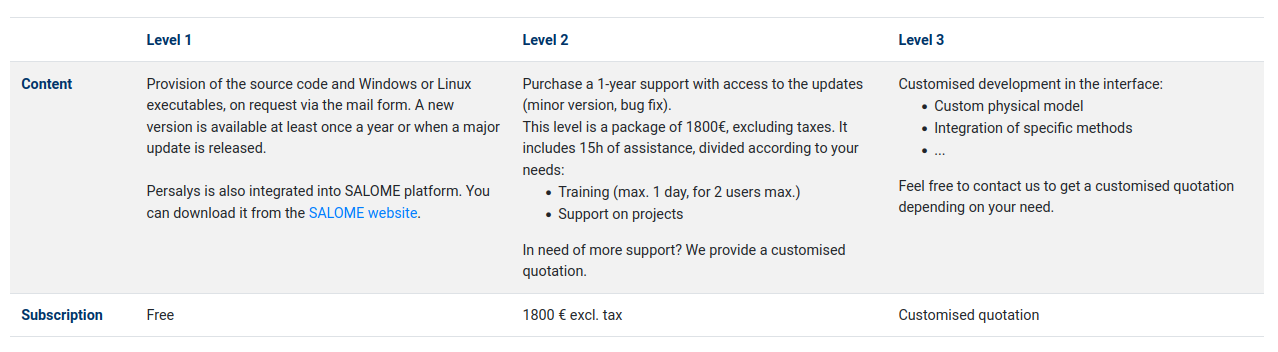
\includegraphics[width=0.6\textwidth]{figures/site.png}
\end{center}

\end{frame}

%%%%%%%%%%%%%%%%%%%%%%%%%%%%%%%%

\begin{frame}
  \frametitle{Summary}
  \begin{itemize}
  \item Partners : EDF, Phimeca
  \item Licence : LGPL
  \item Schedule : new release twice a year
  \item Availability :
    \begin{itemize}
    \item Stand-alone version : for free on demand on \url{www.persalys.fr}
    \item SALOME\_EDF in the "CONTRIBUTIONS" section
      since 2018 on \url{https://www.salome-platform.org}
    \item Debian ``bookworm'' \url{https://packages.debian.org/source/bookworm/persalys} \\
      We thank Pierre Gruet (EDF) for this outstanding work!
    \end{itemize}
  \end{itemize}
\end{frame}

\section{What's new?}

\begin{frame}
  \frametitle{Stepwise linear model - Definition}
  \begin{itemize}
    \item Uses \url{LinearModelStepwiseAlgorithm} from OpenTURNS
    \item From a design of experiment or a data model
  \end{itemize}

  \begin{columns}
    \column{0.1\textwidth}

    \column{0.4\textwidth}
    \begin{center}
      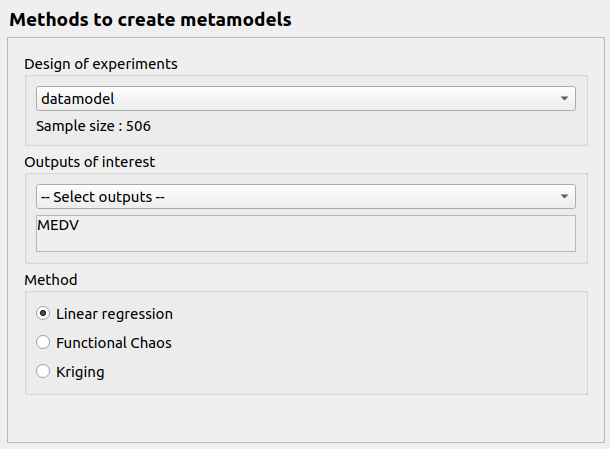
\includegraphics[width=\textwidth]{figures/linearModel1.png}
    \end{center}

    \column{0.4\textwidth}
    \begin{center}
      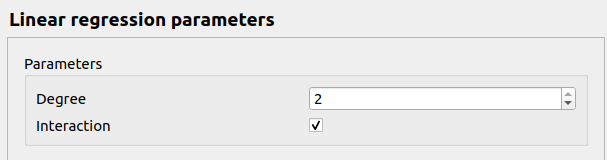
\includegraphics[width=\textwidth]{figures/linearModel2.png}
      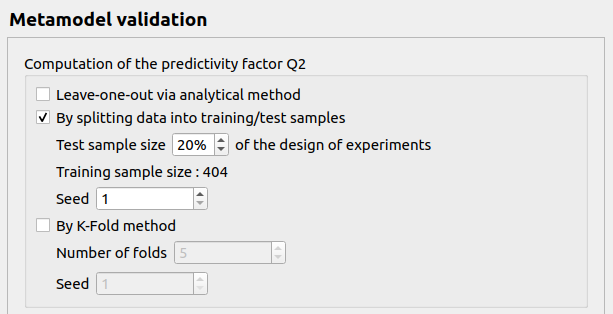
\includegraphics[width=\textwidth]{figures/linearModel2-1.png}
    \end{center}

    \column{0.1\textwidth}
  \end{columns}
  \begin{center}
    \vfill
    \tiny{\url{http://openturns.github.io/openturns/latest/user_manual/response_surface/_generated/openturns.LinearModelStepwiseAlgorithm.html}}
  \end{center}
\end{frame}

%%%%%%%%%%%%%%%%%%%%%%%%%%%%%%%%%%%%%%%%%%%%%%%%%%%%%%%%%%%%%%%%%%%%%%%%%%%%%

\begin{frame}
  \frametitle{Stepwise linear model - Results and validation}

  \begin{columns}
    \column{0.05\textwidth}

    \column{0.25\textwidth}
    \begin{center}
      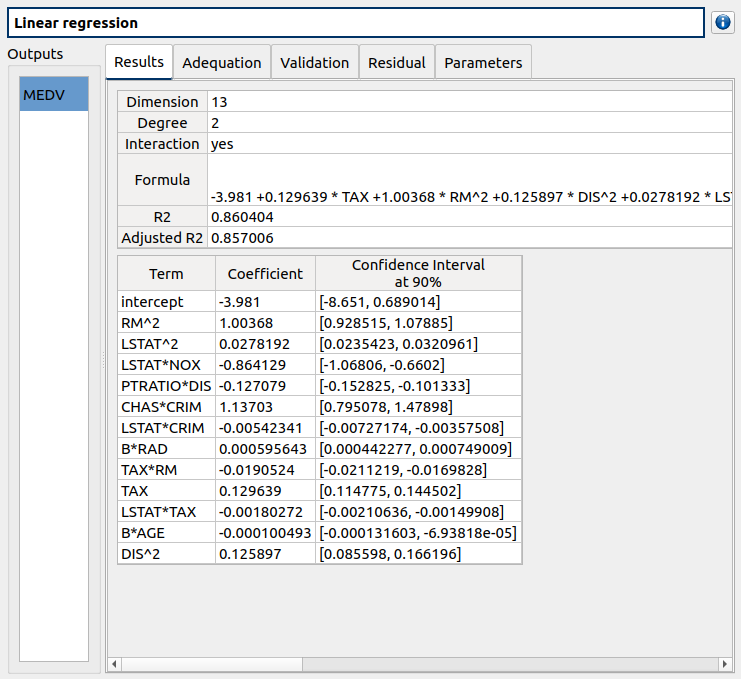
\includegraphics[width=\textwidth]{figures/linearModel3.png}
      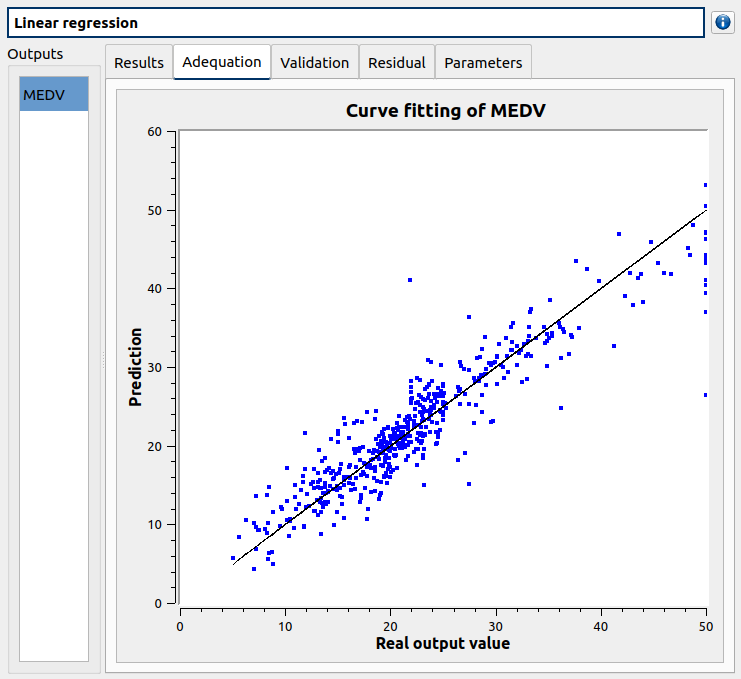
\includegraphics[width=\textwidth]{figures/linearModel4.png}
    \end{center}

    \column{0.05\textwidth}

    \column{0.25\textwidth}
    \begin{center}
      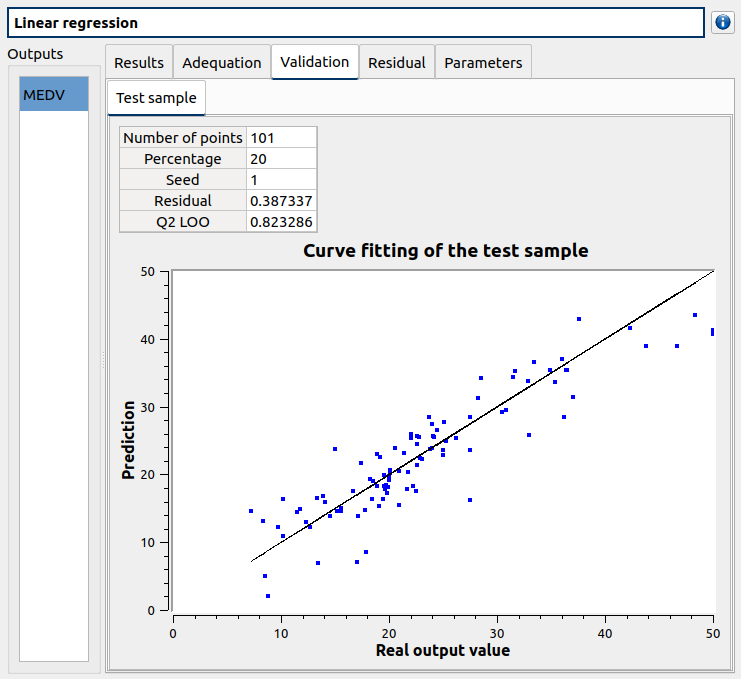
\includegraphics[width=\textwidth]{figures/linearModel5.png}
      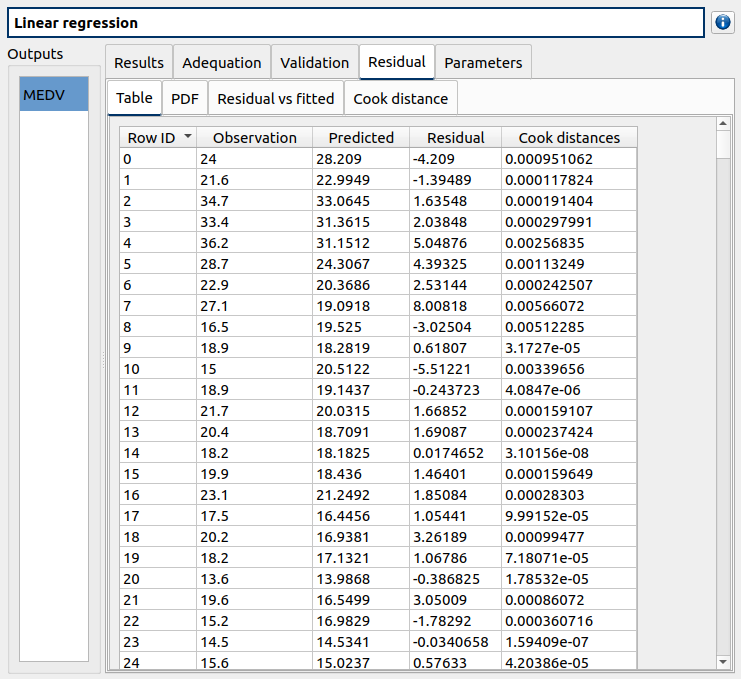
\includegraphics[width=\textwidth]{figures/linearModel6.png}
    \end{center}

    \column{0.05\textwidth}

    \column{0.25\textwidth}
    \begin{center}
      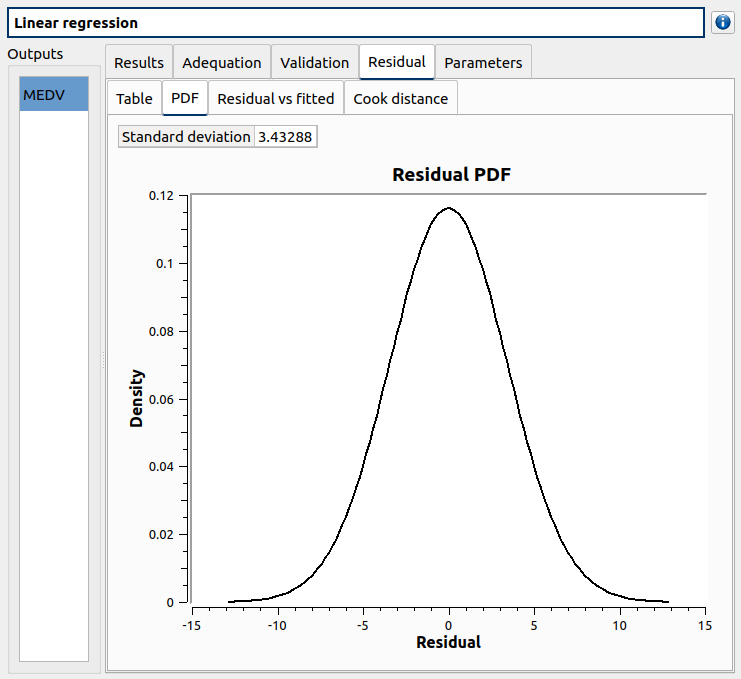
\includegraphics[width=\textwidth]{figures/linearModel7.png}
      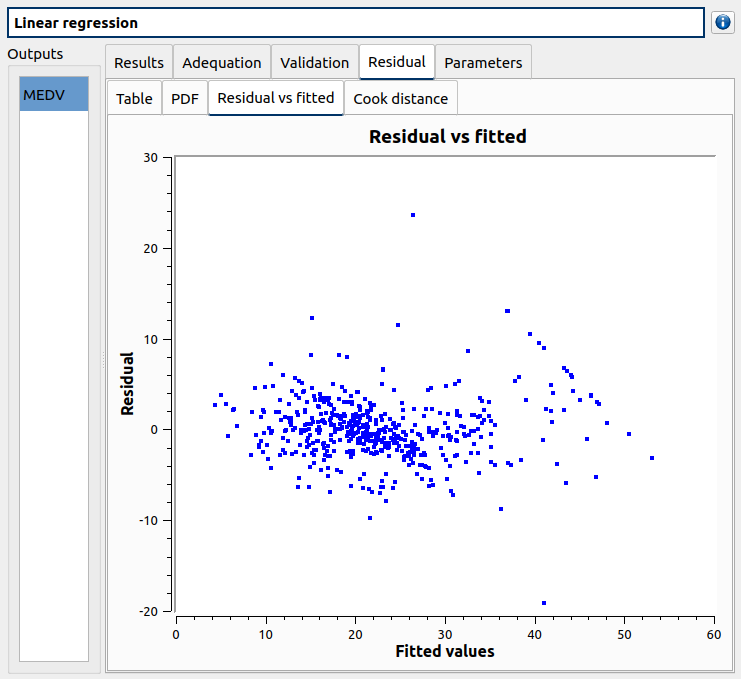
\includegraphics[width=\textwidth]{figures/linearModel8.png}
    \end{center}

    \column{0.05\textwidth}
  \end{columns}
\end{frame}

%%%%%%%%%%%%%%%%%%%%%%%%%%%%%%%%%%%%%%%%%%%%%%%%%%%%%%%%%%%%%%%%%%%%%%%%%%%%%

\begin{frame}
  \frametitle{Optimization overhaul (1)}
   \begin{itemize}
   \item Added constraints support
   \item Added variable type definition for mixed optimization
   \end{itemize}
   \begin{center}
     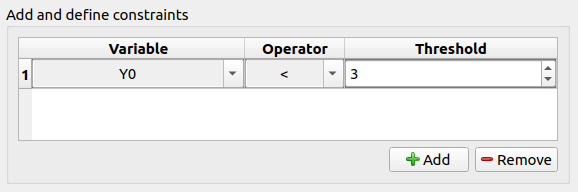
\includegraphics[width=0.5\textwidth]{figures/optimCstr.png} 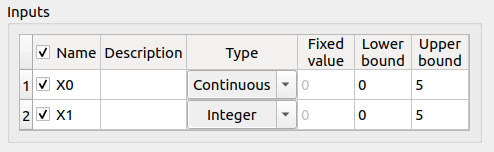
\includegraphics[width=0.5\textwidth]{figures/optimVarTypes.png}
  \end{center}
\end{frame}

%%%%%%%%%%%%%%%%%%%%%%%%%%%%%%%%%%%%%%%%%%%%%%%%%%%%%%%%%%%%%%%%%%%%%%%%%%%%%

\begin{frame}
  \frametitle{Optimization overhaul (2)}

  \begin{itemize}
  \item Added multi-objective optimization analysis \\
    As a service for NavalGroup \\
    Evolutionary algorithms from \url{Pagmo}
  \end{itemize}

  \begin{columns}
    \column{0.02\textwidth}

    \column{0.16\textwidth}
    \begin{center}
      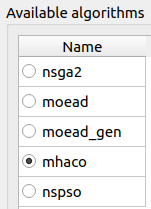
\includegraphics[width=0.8\textwidth]{figures/moAlgos.png}
    \end{center}

    \column{0.4\textwidth}
    \begin{center}
      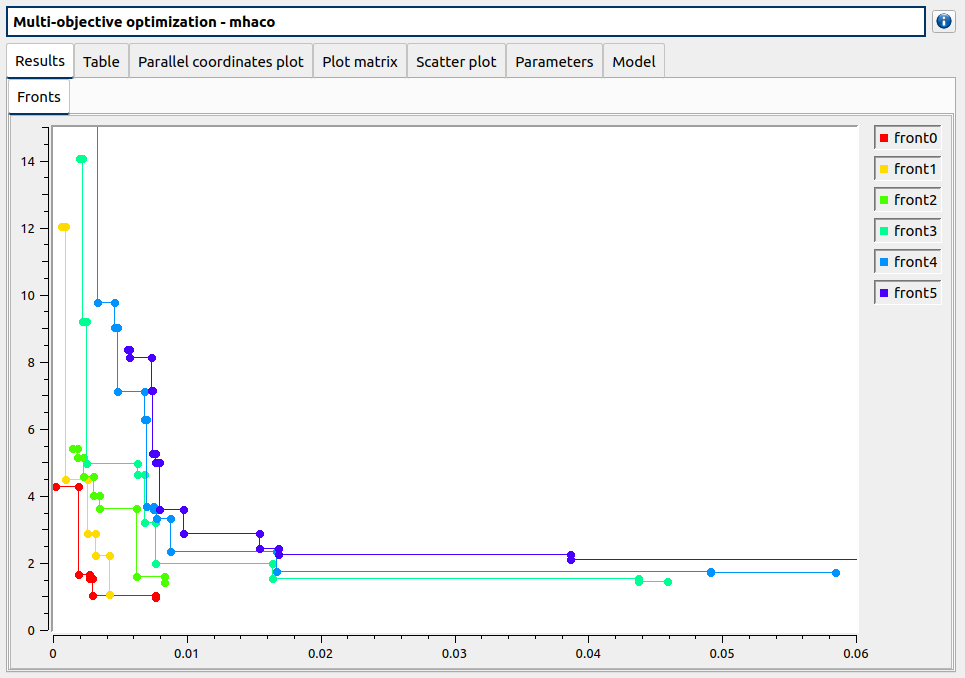
\includegraphics[width=\textwidth]{figures/pareto_front.png}
    \end{center}

    \column{0.4\textwidth}
    \begin{center}
      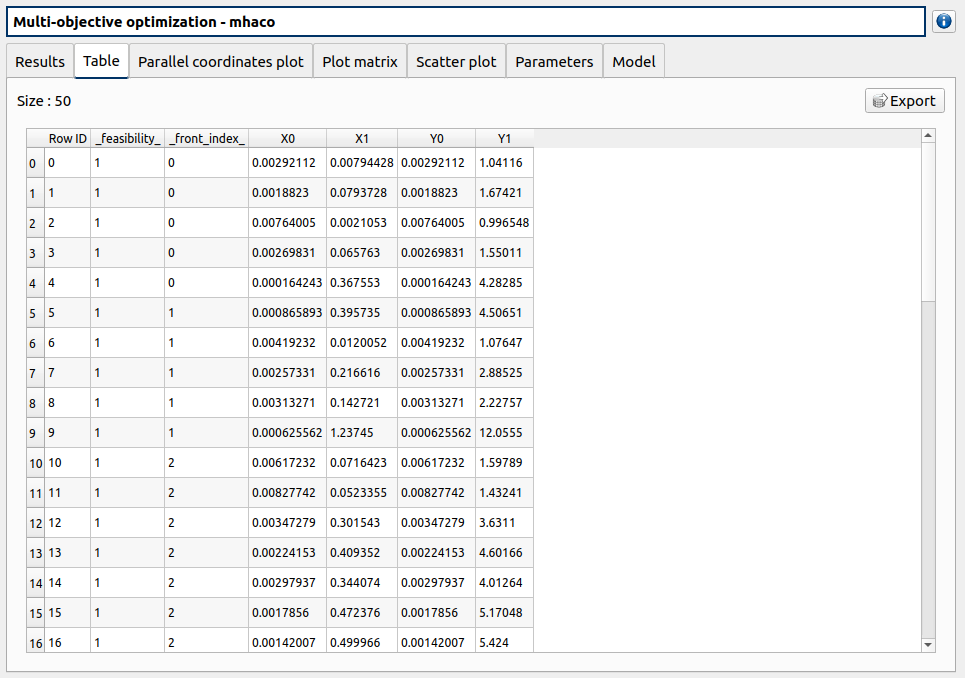
\includegraphics[width=\textwidth]{figures/moResults.png}
    \end{center}

    \column{0.02\textwidth}
  \end{columns}
  \begin{center}
    \vfill
    \tiny{\url{https://esa.github.io/pagmo2/}}
  \end{center}
\end{frame}

%%%%%%%%%%%%%%%%%%%%%%%%%%%%%%%%%%%%%%%%%%%%%%%%%%%%%%%%%%%%%%%%%%%%%%%%%%%%%

\begin{frame}
  \frametitle{Miscellaneous features}
   \begin{itemize}
   \item Sampling using existing data
   \end{itemize}
   \begin{center}
     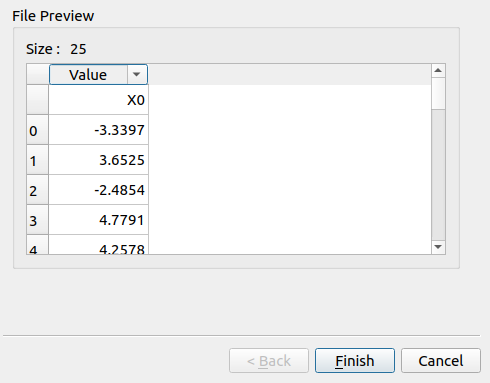
\includegraphics[height=0.3\textheight]{figures/userDef1.png} 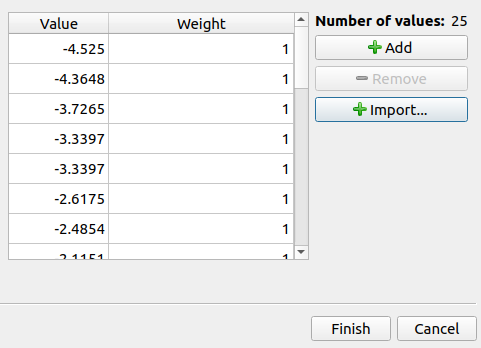
\includegraphics[height=0.3\textheight]{figures/userDef2.png} 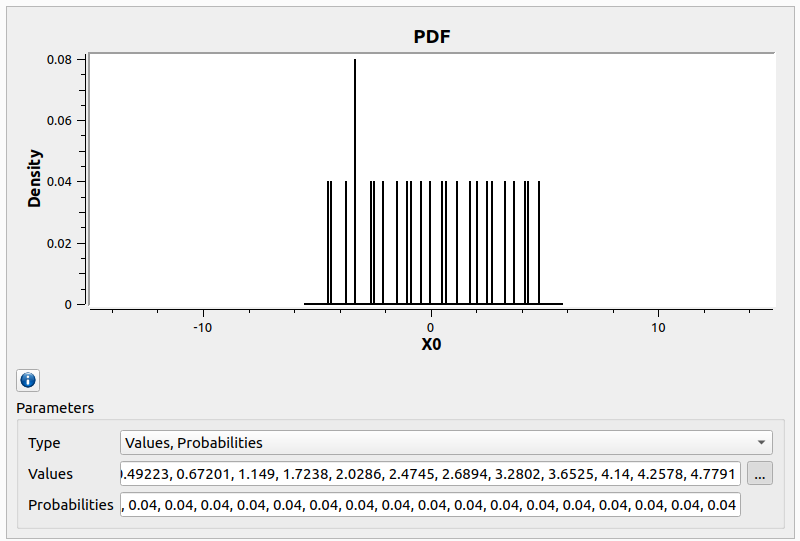
\includegraphics[height=0.3\textheight]{figures/userDef3.png}
   \end{center}
   \begin{itemize}
   \item NormalCopula can be parametrised w. shape and Kendall matrices (only Spearman was available)
   \end{itemize}


%   \begin{columns}
%     \column{0.05\textwidth}
%     \column{0.45\textwidth}
%     \begin{center}
%       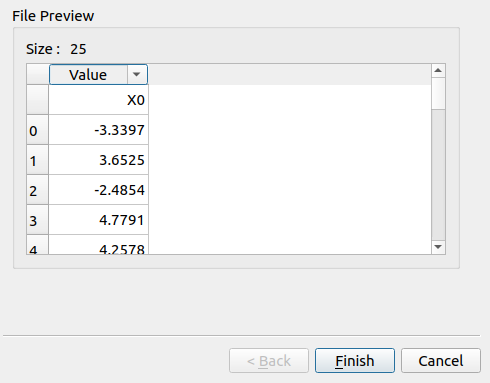
\includegraphics[width=0.5\textwidth]{figures/userDef1.png}
%     \end{center}
%
%     \column{0.45\textwidth}
%     \begin{center}
%       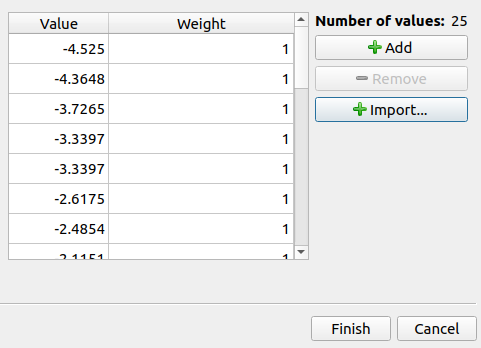
\includegraphics[width=0.5\textwidth]{figures/userDef2.png}
%     \end{center}
%     \column{0.05\textwidth}
%   \end{columns}
\end{frame}

%%%%%%%%%%%%%%%%%%%%%%%%%%%%%%%%%%%%%%%%%%%%%%%%%%%%%%%%%%%%%%%%%%%%%%%%%%%%%

\begin{frame}
  \frametitle{Miscellaneous features}
  \begin{columns}
    \column{0.5\textwidth}
    \begin{itemize}
    \item Coupling model command environment override
    \end{itemize}
    \column{0.5\textwidth}
    \begin{center}
      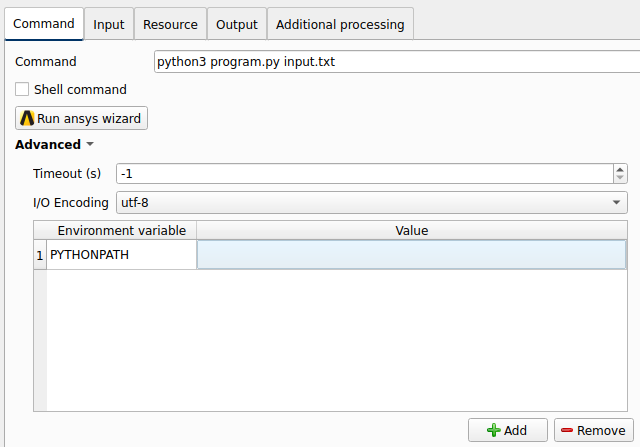
\includegraphics[height=0.3\textheight]{figures/couplingEnv.png}
    \end{center}
  \end{columns}

  \begin{columns}
    \column{0.5\textwidth}
    \begin{itemize}
    \item Gradient evaluation
    \end{itemize}
    \column{0.5\textwidth}
    \begin{center}
      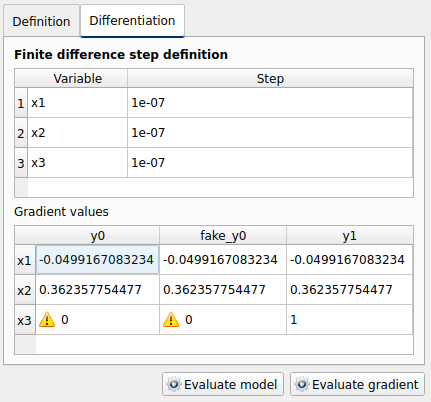
\includegraphics[height=0.3\textheight]{figures/gradient.png}
    \end{center}
  \end{columns}
\end{frame}

%%%%%%%%%%%%%%%%%%%%%

\begin{frame}
  \begin{columns}
    \column{0.4\textwidth}
    \begin{itemize}
    \item Inference :
      \begin{itemize}
      \item Optional distribution parameters confidence interval estimation
      \item Lilliefors fitting test (only Kolmogorov-Smirnov was available)
      \end{itemize}
    \end{itemize}
    \column{0.6\textwidth}
    \begin{center}
      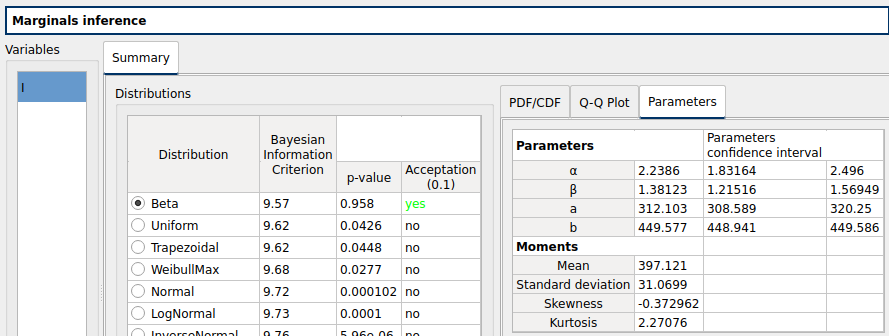
\includegraphics[height=0.3\textheight]{figures/inference.png}
    \end{center}
  \end{columns}

  \begin{columns}
    \column{0.4\textwidth}
    \begin{itemize}
    \item Design of experiment error handling
    \end{itemize}
    \column{0.6\textwidth}
    \begin{center}
      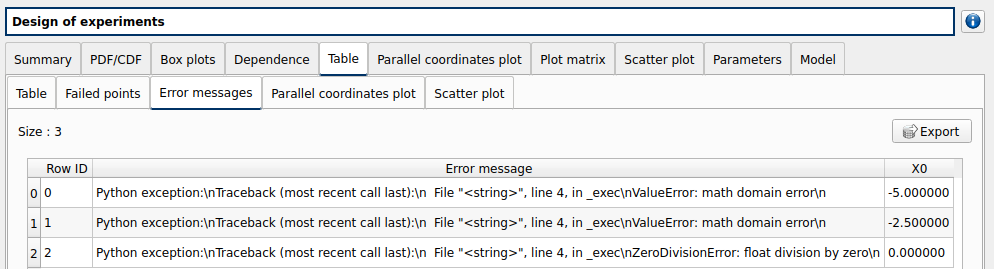
\includegraphics[height=0.3\textheight]{figures/errorDesc.png}
    \end{center}
  \end{columns}
\end{frame}

%%%%%%%%%%%%%%%%%%%%%%%%%%%%%%%%%%%%%%%%%%%%%%%%%%%%%%%%%%%%%%%%%%%%%%%%%%%%%

\begin{frame}
  \frametitle{Miscellaneous features}
    \begin{columns}
    \column{0.99\textwidth}
    \begin{itemize}
    \item Confidence interval length as analysis stopping criterion
    \item Sample tables partial copy pasting
    \item Ansys intermediate parameters detection
    \end{itemize}
    \vspace{30px}
    \begin{itemize}
    \item Coming soon
      \begin{itemize}
      \item Data field model \\
        Import model mesh and data from already evaluated firld samples
      \item Calibration QQ-plots
      \end{itemize}
    \end{itemize}
    \column{0.01\textwidth}
  \end{columns}
\end{frame}

%%%%%%%%%%%%%%%%%%%%%%%%%%%%%%%%%%%%%%%%%%%%%%%%%%%%%%%%%%%%%%%%%%%%%%%%%%%%%

\section{What's next?}
\begin{frame}
  \begin{itemize}
  \item Design of experiments overhaul
  \item Detach-attach jobs on distant cluster - interrupt (instantly) running analysis
  \item Python/YACS physical models merge
  \end{itemize}
\end{frame}

%%%%%%%%%%%%%%%%%%%%%%%%%%%%%%%%%%%%%%%%%%%%%%%%%%%%%%%%%%%%%%%%%%%%%%%%%%%%%
\begin{frame}
\frametitle{The end}
\begin{center}
Thanks !
\end{center}

\begin{center}
Questions ?
\end{center}

\end{frame}

\note{
Thank you for your attention.

If you have any question, it would be a pleasure to answer them.

If you want a live demo of PERSALYS, we can show you during the coffee break.
}

% %%%%%%%%%%%%%%%%%%%%%%%%%%%%%%%%%%%%%%%%%%%%%%%%%%%%%%%%%%%%%%%%%%%%%%%%%%%%%

\end{document}
